\documentclass[11pt, oneside]{article}
\usepackage{titling, geometry, hyperref, algorithm}
\usepackage{amsmath, amssymb, amsthm}              % mathematical packages
\usepackage{graphicx, caption, subcaption}         % images
\usepackage{textcomp, CJKutf8}                     % misc. text formatting
\usepackage{tikz, pgfplots, tikz-network}          % plots and graphs
\usepackage[noend]{algpseudocode}                  % algorithm psuedocode
\usepackage[cache=true]{minted}                    % source code
\usepackage[style=numeric, sorting=none]{biblatex} % bibliography
\geometry{a4paper}

\hypersetup{
  colorlinks=true,
  urlcolor=cyan
}

% https://tex.stackexchange.com/questions/343494/minted-red-box-around-greek-characters
\makeatletter
\AtBeginEnvironment{minted}{\dontdofcolorbox}
\def\dontdofcolorbox{\renewcommand\fcolorbox[4][]{##4}}
\makeatother

\newcommand{\emphasis}[1]{\textbf{\textit{#1}}}
\graphicspath{{./images/}}
\addbibresource{ref.bib}

\theoremstyle{plain}
\newtheorem{theorem}{Theorem}[section]
\newtheorem{corollary}{Corollary}[theorem]
\newtheorem{lemma}[theorem]{Lemma}

\theoremstyle{definition}
\newtheorem{definition}{Definition}[section]
\renewcommand\qedsymbol{$\square$}

\newcommand{\ve}[1]{\mathbf{#1}}

\title{Eigenvalues of Permutation Matrices}
\author{Stephen Huan}
\date{April 27, 2020}

\begin{document}
\maketitle

\section{Introduction}

\textit{If you are confused, read \href{https://activities.tjhsst.edu/cubing/static/pdfs/Linearization/linear.pdf}{this} first}.

\section{Eigenvalues}

\begin{definition}
The graph representation of permutation matrices.
\end{definition}

Let \( P \) be a permutation matrix and \( \pi \) be a permutation which
represents that matrix. The permutation graph of \( \pi \) is defined
as follows: create a node for each number in \( \pi \).
Then, a directed edge between \( (u, v) \) exists if \( u \)
is in the position that \( v \) occupied before the permutation.
For example, let:
\[ \pi = \begin{pmatrix}
         1 & 2 & 3 & 4 & 5 \\
         3 & 5 & 1 & 2 & 4
        \end{pmatrix}
\]

\begin{figure}[h!]
    \centering
    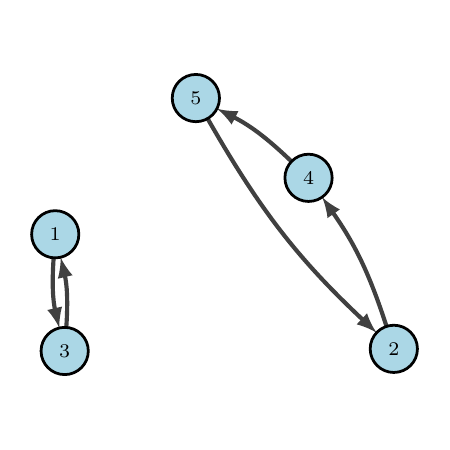
\begin{tikzpicture}
    \clip (0,0) rectangle (5.0,5.0);
    \Vertex[x=0.470,y=0.894,label=3]{3}
    \Vertex[x=2.136,y=4.106,label=5]{5}
    \Vertex[x=0.350,y=2.376,label=1]{1}
    \Vertex[x=4.650,y=0.921,label=2]{2}
    \Vertex[x=3.567,y=3.093,label=4]{4}
    \Edge[,bend=-8.531,Direct](3)(1)
    \Edge[,bend=-8.531,Direct](5)(2)
    \Edge[,bend=-8.531,Direct](1)(3)
    \Edge[,bend=-8.531,Direct](2)(4)
    \Edge[,bend=-8.531,Direct](4)(5)
    \end{tikzpicture}
    \caption{Permutation graph for \( \pi \)}
\end{figure}

Every node in the permutation graph has an indegree of 1 and an outdegree of 1 since
each node can only occupy one position, and, correspondingly,
each position can only be occupied by one node.
\begin{lemma}
Each connected component in the permutation graph must be a cycle,
i.e., a circular linked list such that moving from any node brings
one back to the same node.
\end{lemma}
\begin{proof}
Because the outdegree of each node is 1, there is only one path away from the node.
Suppose for the sake of contradiction that it is possible to start from a node
and never return to that node. Since there are a finite number of nodes,
there must be a cycle in the graph which does not go through the start.
Take the point at which a node not contained in the cycle points to
a node in the cycle. The node in the cycle must have an indegree of two,
since it has a node in the cycle pointing to it and a node outside of the cycle.
This violates the property that every node has an indegree of one,
proving our original assumption is impossible.
\end{proof}

\begin{corollary}
Any permutation can be written as the product of cycles \( C_1 C_2 \ldots C_n \).
\end{corollary}

\begin{theorem}
The real eigenvalues of a permutation matrix can only be 1 or -1.
\end{theorem}

\begin{proof}
Consider the sum of the absolute value of each entry in a vector, which
is invariant under multiplication by a permutation matrix because
a permutation matrix only permutes the order of the entries in a vector,
and addition is commutative. Suppose \( P \) is a permutation matrix,
\( \lambda \) is an eigenvalue, and \( \ve{v} \) is an eigenvector of \( \lambda \).
By the definition of an eigenvalue, \( P = \lambda \ve{v} \).

Computing the sum of the absolute value of each entry in \( \ve{v} \):
\begin{align*}
\sum_{i=1}^n | \lambda \ve{v}_i | &= \sum_{i=1}^n | \ve{v}_i | \\
| \lambda | \sum_{i=1}^n | \ve{v}_i | &= \sum_{i=1}^n | \ve{v}_i | \\
| \lambda | &= 1 \\
\lambda &= -1, 1
\end{align*}
\end{proof}

\begin{lemma}
Every permutation matrix has an eigenvalue of 1.
\end{lemma}

\begin{proof}
Consider a vector of all 1's. Permuting this vector yields the same vector,
so it is an eigenvector of eigenvalue 1 by definition.
\end{proof}

\begin{lemma}
The number of linearly independent eigenvectors for an eigenvalue of 1 for a permutation matrix
is the number of cycles in the corresponding permutation.
\end{lemma}

\begin{proof}
Each cycle is independent of any other cycle, therefore each cycle
is a free variable in the solution to the homogeneous equation \( P - \lambda I \).
The number of free variables determines the number of eigenvectors.
\end{proof}

\begin{lemma}
A permutation matrix has an eigenvalue of -1 if and only if it has at least one even length cycle.
\end{lemma}
\begin{proof}
First, consider the case of an even length cycle. Start at an arbitrary node,
and assign it a value of 1 WLOG. The node that the starting node points to must
now be assigned a value of -1, so that when the starting node exchanges positions
with the node it points to the vector appears to have negated at these two positions.
Continuing the chain, each node is assigned a 1 or -1 value in alternating fashion.
When one reaches the start node again, it will be to assign it a value of 1
because the cycle length is even.

Second, consider an odd length cycle. It is not possible to assign a node
with a value unequal to 0, since assigning the alternating signs will end up
attempting to assign the start node a value negative
of the initially assigned value. Thus, the only way to make odd length cycles
consistent with an eigenvalue of -1 is to assign each node in an odd length
cycle the value 0. If a vector is composed of only odd length cycles, then it will be
the zero vector, which is not an eigenvector by definition.

Therefore, the only way to have an eigenvalue of -1 is if there exists at least
one even length cycle, and if there is at least one even length cycle,
it is possible to construct an eigenvector such that permuting the vector
negates it, as discussed above.
\end{proof}

\begin{lemma}
The number of linearly independent eigenvectors for an eigenvalue of -1 for a permutation matrix
is the number of even length cycles in the permutation.
\end{lemma}

\begin{proof}
Since each element in an odd length cycle must necessarily be 0,
they are not free variables and do not contribute eigenvectors.

The proof for even length cycles follows similar to lemma 4.
\end{proof}

\begin{lemma}
The number of eigenvectors a particular entry contributes is 1 for a cycle length of 1,
1 for a cycle length of 2, and less than 1 for a length greater than 2.
\end{lemma}
\begin{proof}
The only eigenvalues of permutation matrices are 1 and -1 by theorem 2,
so we only need to consider the eigenvectors of eigenvalue 1 and -1.

By lemma 4, eigenvalue 1 contributes the number of eigenvectors equal to
the number of cycles, and by lemma 6, eigenvalue -1 contributes the
number of even length cycles.

Let \( C \) be the cycle length. A cycle of length \( C \) also has \( C \)
entries, so if \( N \) is the number of eigenvectors the cycle contributes,
the number an entry contributes is \( \frac{N}{C} \).

Evaluating for \( C = 1 \), there is 1 cycle and 0 even length cycles so
each entry contributes \( \frac{N}{C} = \frac{1}{1} = 1 \) eigenvectors.
For \( C = 2 \), there is 1 cycle and 1 even length cycle so each entry
contributes \( \frac{N}{C} = \frac{2}{2} = 1 \) eigenvectors.
Finally, for \( C > 2 \), \( N \) is at most 2 and \( C > 2 \), so
\( \frac{N}{C} < 1 \).
\end{proof}

\begin{corollary}
The maximum number of eigenvectors an entry can contribute is 1.
\end{corollary}

\newpage

\begin{lemma}
If \( \pi = C_1 C_2 \ldots C_n \), and each cycle
has a length of \( l_1, l_2, \ldots, l_n \),
then the smallest \( k \) such that \( P_{\pi}^k = I \)
is equal to \( \mathrm{lcm }(l_1, l_2, \ldots, l_n) \).
\end{lemma}
\begin{proof}
Take an arbitrary cycle, and put a pointer at an arbitrary node. Multiplying
by the permutation matrix will move this pointer by one edge to the node
it is directed towards, so it will take the length of the cycle to
reach the start node again. Thus, for some cycle length \( l \) and some power \( k \),
\( P^k = I \) if and only if \( k \mod l \equiv 0 \). For that to be true for each
cycle length, \( k \) must be at least \( \mathrm{lcm }(l_1, l_2, \ldots, l_n) \),
and that is the minimum \( k \) can be for \( k \) to be divisible by each \( l_i \).
\end{proof}

\begin{theorem}
A permutation matrix \( P \) is diagonalizable under \( \mathbb{R} \) if and only if \( P^2 = I \).
\end{theorem}

\begin{proof}
A matrix of dimension \( N \)x\( N \) is diagonalizable if and only if it has \( N \)
linearly independent eigenvectors. There are exactly \( N \) entries,
and because of corollary 7.1, the maximum number of eigenvectors is \( N \).
In order to achieve the upper limit of \( N \), each entry needs to contribute
1 eigenvector. If there is a cycle of length \( > 2 \), then there exists an
entry which contributes less than 1 eigenvector, making it impossible to
achieve \( N \) eigenvectors in total.

Therefore, each cycle must be of length \( \leq 2 \). By lemma 8,
the smallest \( k \) such that \( P^k = I \) is \( \mathrm{lcm }(l_1, l_2, \ldots, l_n) \).
If \( l_i \leq 2 \), then \( k \leq 2 \), so \( k = 1 \) or
\( k = 2 \). In either case, \( P^2 = I \). Working backwards, if
\( P^2 = I \), that implies \( k \leq 2 \) which implies that each cycle
length is \( \leq 2 \), making \( P \) diagonalizable.
\end{proof}

\section{Application}
The common application for diagonalization is fast exponentiation.

\begin{lemma}
The exponentiation of a diagonal matrix is the exponentiation
of each entry on the diagonal.
\end{lemma}
\begin{proof}
Let the inductive hypothesis be that \[ D = \begin{bmatrix}
  d_1 & 0 & \dots & 0 \\
  0 & d_2 & \dots & 0 \\
  \vdots & \vdots & \ddots & \vdots \\
  0 & 0 & \dots & d_n
\end{bmatrix}
\text{ and that }
D^k = \begin{bmatrix}
  d_1^k & 0 & \dots & 0 \\
  0 & d_2^k & \dots & 0 \\
  \vdots & \vdots & \ddots & \vdots \\
  0 & 0 & \dots & d_n^k
\end{bmatrix} \]

\[ D^{k + 1} = D D^k =
\begin{bmatrix}
  d_1 & 0 & \dots & 0 \\
  0 & d_2 & \dots & 0 \\
  \vdots & \vdots & \ddots & \vdots \\
  0 & 0 & \dots & d_n
\end{bmatrix}
\begin{bmatrix}
  d_1^k & 0 & \dots & 0 \\
  0 & d_2^k & \dots & 0 \\
  \vdots & \vdots & \ddots & \vdots \\
  0 & 0 & \dots & d_n^k
\end{bmatrix}
=
\begin{bmatrix}
  d_1^{k + 1} & 0 & \dots & 0 \\
  0 & d_2^{k + 1} & \dots & 0 \\
  \vdots & \vdots & \ddots & \vdots \\
  0 & 0 & \dots & d_n^{k + 1}
\end{bmatrix}
\]

Since \( D^1 \) is equal to each entry on the diagonal being raised
to the first power, the lemma is true for all integer powers \( \geq 1\).
\end{proof}

\begin{corollary}
If exponentiation to the power of \( k \) can be done in \( O(\log k) \),
matrix exponentiation of a diagonal matrix can be done in \( O(n \log k) \).
\end{corollary}

\begin{theorem}
If \( A = P D P^{-1} \), \( A^k = P D^k P^{-1} \).
\end{theorem}
\begin{proof}
Let the inductive hypothesis be that \( A^k = P D^k P^{-1} \). \\
\( A^{k + 1} = A A^{k} = P D P^{-1}(P D^k P^{-1}) = P D^{k + 1} P^{-1} \).

Since \( A^1 \) = \( P D^1 P^{-1} \), the theorem is true for all integer \( k \geq 1 \).
\end{proof}

\begin{corollary}
If matrix multiplication can be done in time \( O(n^z) \),
and \( A = PDP^{-1} \), \( A^k \) can be computed in time \( O(n^z + n \log k ) \)
by corollary 3.1.
\end{corollary}

The lower bound for general matrix multiplication is not known, but an obvious one is
\( O(n^2) \). In general, it is \( O(n^z) \) for some \( 2 \leq z \leq 3 \).
A matrix exponentiation algorithm not relying on diagonalization is given
below, instead using repeated squaring to achieve the same result.
The running time is \( O(n^z \log k) \), which is worse than the
\( O(n^z + n \log k ) \) time given by the diagonalization algorithm.

\begin{algorithm}
\caption{Fast Matrix Exponentiation}
\begin{minted}{python}
def mat_exp(A: np.array, k: int) -> list:
    v = np.identity(len(A))
    while k > 0:
        if k & 1 == 1:
            v = v @ A
        k >>= 1
        A = A @ A
    return v
\end{minted}
\end{algorithm}

However, note that it is possible to multiply
two permutation matrices in \( O(n) \).
Represent each permutation matrix by its permutation \( \pi \)
of length \( n \). The algorithm for multiplying two permutations \( \pi_1 \)
and \( \pi_2 \) is then as follows: initialize an empty list.
Then, going over each element \( e \) of \( \pi_2 \),
append the value of \( \pi_1 \) at index \( e \) to the list.

\begin{algorithm}
\caption{Permutation Multiplication}
\begin{minted}{python}
def mult(l1: list, l2: list) -> list:
    return [l1[n] for n in l2]
\end{minted}
\end{algorithm}

Using this as a backend for repeated squaring, the final algorithm has a runtime
of \( O(n \log k + n^2) \), where the \( n^2 \) term is a result of
turning a permutation into a permutation matrix and can be turned into
\( O(n \log k) \) if one is willing to modify the original matrix.
In diagonalization, however, one still needs to do general matrix multiplications,
making the running time \( O(n \log k + n^z) \) asymptotically worse.

\printbibliography
\end{document}
